\documentclass[twoside]{book}

% Packages required by doxygen
\usepackage{fixltx2e}
\usepackage{calc}
\usepackage{doxygen}
\usepackage[export]{adjustbox} % also loads graphicx
\usepackage{graphicx}
\usepackage[utf8]{inputenc}
\usepackage{makeidx}
\usepackage{multicol}
\usepackage{multirow}
\PassOptionsToPackage{warn}{textcomp}
\usepackage{textcomp}
\usepackage[nointegrals]{wasysym}
\usepackage[table]{xcolor}

% Font selection
\usepackage[T1]{fontenc}
\usepackage[scaled=.90]{helvet}
\usepackage{courier}
\usepackage{amssymb}
\usepackage{sectsty}
\renewcommand{\familydefault}{\sfdefault}
\allsectionsfont{%
  \fontseries{bc}\selectfont%
  \color{darkgray}%
}
\renewcommand{\DoxyLabelFont}{%
  \fontseries{bc}\selectfont%
  \color{darkgray}%
}
\newcommand{\+}{\discretionary{\mbox{\scriptsize$\hookleftarrow$}}{}{}}

% Page & text layout
\usepackage{geometry}
\geometry{%
  a4paper,%
  top=2.5cm,%
  bottom=2.5cm,%
  left=2.5cm,%
  right=2.5cm%
}
\tolerance=750
\hfuzz=15pt
\hbadness=750
\setlength{\emergencystretch}{15pt}
\setlength{\parindent}{0cm}
\setlength{\parskip}{3ex plus 2ex minus 2ex}
\makeatletter
\renewcommand{\paragraph}{%
  \@startsection{paragraph}{4}{0ex}{-1.0ex}{1.0ex}{%
    \normalfont\normalsize\bfseries\SS@parafont%
  }%
}
\renewcommand{\subparagraph}{%
  \@startsection{subparagraph}{5}{0ex}{-1.0ex}{1.0ex}{%
    \normalfont\normalsize\bfseries\SS@subparafont%
  }%
}
\makeatother

% Headers & footers
\usepackage{fancyhdr}
\pagestyle{fancyplain}
\fancyhead[LE]{\fancyplain{}{\bfseries\thepage}}
\fancyhead[CE]{\fancyplain{}{}}
\fancyhead[RE]{\fancyplain{}{\bfseries\leftmark}}
\fancyhead[LO]{\fancyplain{}{\bfseries\rightmark}}
\fancyhead[CO]{\fancyplain{}{}}
\fancyhead[RO]{\fancyplain{}{\bfseries\thepage}}
\fancyfoot[LE]{\fancyplain{}{}}
\fancyfoot[CE]{\fancyplain{}{}}
\fancyfoot[RE]{\fancyplain{}{\bfseries\scriptsize Generated by Doxygen }}
\fancyfoot[LO]{\fancyplain{}{\bfseries\scriptsize Generated by Doxygen }}
\fancyfoot[CO]{\fancyplain{}{}}
\fancyfoot[RO]{\fancyplain{}{}}
\renewcommand{\footrulewidth}{0.4pt}
\renewcommand{\chaptermark}[1]{%
  \markboth{#1}{}%
}
\renewcommand{\sectionmark}[1]{%
  \markright{\thesection\ #1}%
}

% Indices & bibliography
\usepackage{natbib}
\usepackage[titles]{tocloft}
\setcounter{tocdepth}{3}
\setcounter{secnumdepth}{5}
\makeindex

% Hyperlinks (required, but should be loaded last)
\usepackage{ifpdf}
\ifpdf
  \usepackage[pdftex,pagebackref=true]{hyperref}
\else
  \usepackage[ps2pdf,pagebackref=true]{hyperref}
\fi
\hypersetup{%
  colorlinks=true,%
  linkcolor=blue,%
  citecolor=blue,%
  unicode%
}

% Custom commands
\newcommand{\clearemptydoublepage}{%
  \newpage{\pagestyle{empty}\cleardoublepage}%
}

\usepackage{caption}
\captionsetup{labelsep=space,justification=centering,font={bf},singlelinecheck=off,skip=4pt,position=top}

%===== C O N T E N T S =====

\begin{document}

% Titlepage & ToC
\hypersetup{pageanchor=false,
             bookmarksnumbered=true,
             pdfencoding=unicode
            }
\pagenumbering{roman}
\begin{titlepage}
\vspace*{7cm}
\begin{center}%
{\Large lab8 }\\
\vspace*{1cm}
{\large Generated by Doxygen 1.8.11}\\
\end{center}
\end{titlepage}
\clearemptydoublepage
\tableofcontents
\clearemptydoublepage
\pagenumbering{arabic}
\hypersetup{pageanchor=true}

%--- Begin generated contents ---
\chapter{Class Index}
\section{Class List}
Here are the classes, structs, unions and interfaces with brief descriptions\+:\begin{DoxyCompactList}
\item\contentsline{section}{\hyperlink{structmatan}{matan} \\*Defines a tasks matan type }{\pageref{structmatan}}{}
\item\contentsline{section}{\hyperlink{structRequest}{Request} \\*Defines a \hyperlink{structRequest}{Request} data type }{\pageref{structRequest}}{}
\end{DoxyCompactList}

\chapter{File Index}
\section{File List}
Here is a list of all documented files with brief descriptions\+:\begin{DoxyCompactList}
\item\contentsline{section}{include/\hyperlink{matan_8h}{matan.\+h} \\*Matan type , it`s parsing and general tasks }{\pageref{matan_8h}}{}
\item\contentsline{section}{include/\hyperlink{request_8h}{request.\+h} \\*\hyperlink{structRequest}{Request} type and its parsing }{\pageref{request_8h}}{}
\end{DoxyCompactList}

\chapter{Class Documentation}
\hypertarget{structmatan}{}\section{matan Struct Reference}
\label{structmatan}\index{matan@{matan}}


defines a tasks matan type  




{\ttfamily \#include $<$matan.\+h$>$}

\subsection*{Public Attributes}
\begin{DoxyCompactItemize}
\item 
char {\bfseries name} \mbox{[}100\mbox{]}\hypertarget{structmatan_ac50516d5800781ea80f361bf268cee21}{}\label{structmatan_ac50516d5800781ea80f361bf268cee21}

\item 
int {\bfseries id}\hypertarget{structmatan_ac68eae3b7f0955c4c10256d7a529c595}{}\label{structmatan_ac68eae3b7f0955c4c10256d7a529c595}

\end{DoxyCompactItemize}


\subsection{Detailed Description}
defines a tasks matan type 

The documentation for this struct was generated from the following file\+:\begin{DoxyCompactItemize}
\item 
include/\hyperlink{matan_8h}{matan.\+h}\end{DoxyCompactItemize}

\hypertarget{structRequest}{}\section{Request Struct Reference}
\label{structRequest}\index{Request@{Request}}


defines a \hyperlink{structRequest}{Request} data type  




{\ttfamily \#include $<$request.\+h$>$}

\subsection*{Public Attributes}
\begin{DoxyCompactItemize}
\item 
char {\bfseries command} \mbox{[}100\mbox{]}\hypertarget{structRequest_ab89e3bcf634e4dfe1a1fc7b4397114c0}{}\label{structRequest_ab89e3bcf634e4dfe1a1fc7b4397114c0}

\item 
char {\bfseries data} \mbox{[}100\mbox{]}\hypertarget{structRequest_a2a47f13762766a469a1eb5a1489daf41}{}\label{structRequest_a2a47f13762766a469a1eb5a1489daf41}

\end{DoxyCompactItemize}


\subsection{Detailed Description}
defines a \hyperlink{structRequest}{Request} data type 

The documentation for this struct was generated from the following file\+:\begin{DoxyCompactItemize}
\item 
include/\hyperlink{request_8h}{request.\+h}\end{DoxyCompactItemize}

\chapter{File Documentation}
\hypertarget{matan_8h}{}\section{include/matan.h File Reference}
\label{matan_8h}\index{include/matan.\+h@{include/matan.\+h}}


Matan type , it`s parsing and general tasks.  


{\ttfamily \#include $<$string.\+h$>$}\\*
{\ttfamily \#include $<$stdio.\+h$>$}\\*
{\ttfamily \#include $<$assert.\+h$>$}\\*
{\ttfamily \#include $<$jansson.\+h$>$}\\*
{\ttfamily \#include $<$list.\+h$>$}\\*
{\ttfamily \#include $<$libxml/parser.\+h$>$}\\*
{\ttfamily \#include $<$libxml/tree.\+h$>$}\\*
{\ttfamily \#include $<$matan.\+h$>$}\\*
{\ttfamily \#include $<$time.\+h$>$}\\*
Include dependency graph for matan.\+h\+:
\nopagebreak
\begin{figure}[H]
\begin{center}
\leavevmode
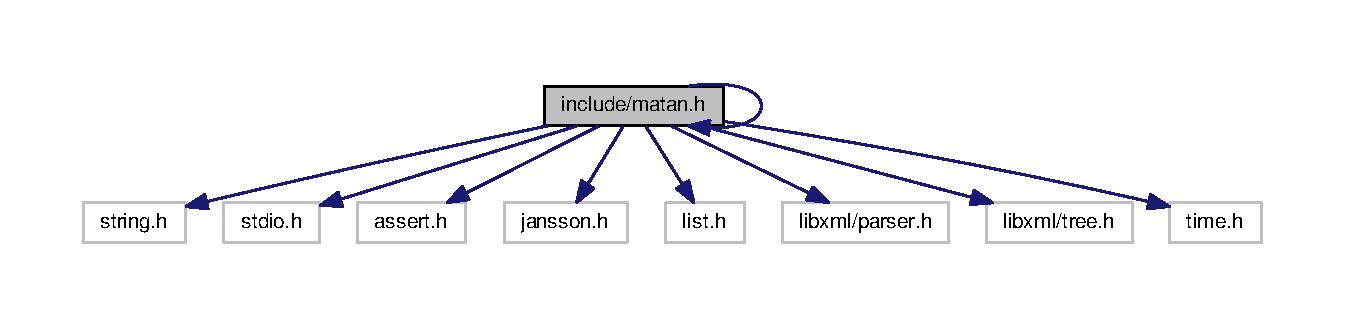
\includegraphics[width=350pt]{matan_8h__incl}
\end{center}
\end{figure}
This graph shows which files directly or indirectly include this file\+:
\nopagebreak
\begin{figure}[H]
\begin{center}
\leavevmode
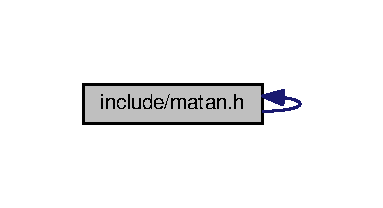
\includegraphics[width=184pt]{matan_8h__dep__incl}
\end{center}
\end{figure}
\subsection*{Classes}
\begin{DoxyCompactItemize}
\item 
struct \hyperlink{structmatan}{matan}
\begin{DoxyCompactList}\small\item\em defines a tasks matan type \end{DoxyCompactList}\end{DoxyCompactItemize}
\subsection*{Functions}
\begin{DoxyCompactItemize}
\item 
char $\ast$ \hyperlink{matan_8h_ae63c72e940f793050744c6a702cd5bb2}{parse\+All\+Json} (List $\ast$list)
\begin{DoxyCompactList}\small\item\em Parsing all matan structures into json. \end{DoxyCompactList}\item 
char $\ast$ \hyperlink{matan_8h_aa2d30a696077eaeadaefcb27d300a3b9}{parse\+Matan\+Request} (char $\ast$str, List $\ast$mat)
\begin{DoxyCompactList}\small\item\em Parsing matan structures into json. \end{DoxyCompactList}\item 
char $\ast$ \hyperlink{matan_8h_a002524c67a53d7ac5af320f061d0fe70}{parse\+Id\+Request} (char $\ast$str, List $\ast$mat)
\begin{DoxyCompactList}\small\item\em Parsing matan structures into json. \end{DoxyCompactList}\item 
char $\ast$ \hyperlink{matan_8h_a6a0a8b58c4f4bffdf1de623afcb1aff2}{file} ()
\begin{DoxyCompactList}\small\item\em file reader \end{DoxyCompactList}\item 
char $\ast$ \hyperlink{matan_8h_a9b6e64fe3a1c278517092bc7614d4fa1}{file\+Data} ()
\begin{DoxyCompactList}\small\item\em file reader and task \end{DoxyCompactList}\item 
char $\ast$ \hyperlink{matan_8h_aee5d32587b4a92a9c971ef7ad266ba09}{Default} ()
\begin{DoxyCompactList}\small\item\em creating default server output \end{DoxyCompactList}\end{DoxyCompactItemize}


\subsection{Detailed Description}
Matan type , it`s parsing and general tasks. 



\subsection{Function Documentation}
\index{matan.\+h@{matan.\+h}!Default@{Default}}
\index{Default@{Default}!matan.\+h@{matan.\+h}}
\subsubsection[{\texorpdfstring{Default()}{Default()}}]{\setlength{\rightskip}{0pt plus 5cm}char$\ast$ Default (
\begin{DoxyParamCaption}
{}
\end{DoxyParamCaption}
)}\hypertarget{matan_8h_aee5d32587b4a92a9c971ef7ad266ba09}{}\label{matan_8h_aee5d32587b4a92a9c971ef7ad266ba09}


creating default server output 

\begin{DoxyReturn}{Returns}
json string with default server parameteres 
\end{DoxyReturn}
\index{matan.\+h@{matan.\+h}!file@{file}}
\index{file@{file}!matan.\+h@{matan.\+h}}
\subsubsection[{\texorpdfstring{file()}{file()}}]{\setlength{\rightskip}{0pt plus 5cm}char$\ast$ file (
\begin{DoxyParamCaption}
{}
\end{DoxyParamCaption}
)}\hypertarget{matan_8h_a6a0a8b58c4f4bffdf1de623afcb1aff2}{}\label{matan_8h_a6a0a8b58c4f4bffdf1de623afcb1aff2}


file reader 

\begin{DoxyReturn}{Returns}
json string with file data 
\end{DoxyReturn}
\index{matan.\+h@{matan.\+h}!file\+Data@{file\+Data}}
\index{file\+Data@{file\+Data}!matan.\+h@{matan.\+h}}
\subsubsection[{\texorpdfstring{file\+Data()}{fileData()}}]{\setlength{\rightskip}{0pt plus 5cm}char$\ast$ file\+Data (
\begin{DoxyParamCaption}
{}
\end{DoxyParamCaption}
)}\hypertarget{matan_8h_a9b6e64fe3a1c278517092bc7614d4fa1}{}\label{matan_8h_a9b6e64fe3a1c278517092bc7614d4fa1}


file reader and task 

\begin{DoxyReturn}{Returns}
json string with file data task 
\end{DoxyReturn}
\index{matan.\+h@{matan.\+h}!parse\+All\+Json@{parse\+All\+Json}}
\index{parse\+All\+Json@{parse\+All\+Json}!matan.\+h@{matan.\+h}}
\subsubsection[{\texorpdfstring{parse\+All\+Json(\+List $\ast$list)}{parseAllJson(List *list)}}]{\setlength{\rightskip}{0pt plus 5cm}char$\ast$ parse\+All\+Json (
\begin{DoxyParamCaption}
\item[{List $\ast$}]{list}
\end{DoxyParamCaption}
)}\hypertarget{matan_8h_ae63c72e940f793050744c6a702cd5bb2}{}\label{matan_8h_ae63c72e940f793050744c6a702cd5bb2}


Parsing all matan structures into json. 


\begin{DoxyParams}{Parameters}
{\em list} & -\/ default list of matan structures \\
\hline
\end{DoxyParams}
\begin{DoxyReturn}{Returns}
json string 
\end{DoxyReturn}
\index{matan.\+h@{matan.\+h}!parse\+Id\+Request@{parse\+Id\+Request}}
\index{parse\+Id\+Request@{parse\+Id\+Request}!matan.\+h@{matan.\+h}}
\subsubsection[{\texorpdfstring{parse\+Id\+Request(char $\ast$str, List $\ast$mat)}{parseIdRequest(char *str, List *mat)}}]{\setlength{\rightskip}{0pt plus 5cm}char$\ast$ parse\+Id\+Request (
\begin{DoxyParamCaption}
\item[{char $\ast$}]{str, }
\item[{List $\ast$}]{mat}
\end{DoxyParamCaption}
)}\hypertarget{matan_8h_a002524c67a53d7ac5af320f061d0fe70}{}\label{matan_8h_a002524c67a53d7ac5af320f061d0fe70}


Parsing matan structures into json. 


\begin{DoxyParams}{Parameters}
{\em mat} & -\/ default list of matan structures \\
\hline
{\em str} & -\/ user parametric request \\
\hline
\end{DoxyParams}
\begin{DoxyReturn}{Returns}
json string 
\end{DoxyReturn}
\index{matan.\+h@{matan.\+h}!parse\+Matan\+Request@{parse\+Matan\+Request}}
\index{parse\+Matan\+Request@{parse\+Matan\+Request}!matan.\+h@{matan.\+h}}
\subsubsection[{\texorpdfstring{parse\+Matan\+Request(char $\ast$str, List $\ast$mat)}{parseMatanRequest(char *str, List *mat)}}]{\setlength{\rightskip}{0pt plus 5cm}char$\ast$ parse\+Matan\+Request (
\begin{DoxyParamCaption}
\item[{char $\ast$}]{str, }
\item[{List $\ast$}]{mat}
\end{DoxyParamCaption}
)}\hypertarget{matan_8h_aa2d30a696077eaeadaefcb27d300a3b9}{}\label{matan_8h_aa2d30a696077eaeadaefcb27d300a3b9}


Parsing matan structures into json. 


\begin{DoxyParams}{Parameters}
{\em mat} & -\/ default list of matan structures \\
\hline
{\em str} & -\/ user parametric request \\
\hline
\end{DoxyParams}
\begin{DoxyReturn}{Returns}
json string 
\end{DoxyReturn}

\hypertarget{request_8h}{}\section{include/request.h File Reference}
\label{request_8h}\index{include/request.\+h@{include/request.\+h}}


\hyperlink{structRequest}{Request} type and its parsing.  


{\ttfamily \#include $<$ctype.\+h$>$}\\*
{\ttfamily \#include $<$string.\+h$>$}\\*
{\ttfamily \#include $<$stdlib.\+h$>$}\\*
{\ttfamily \#include $<$stdio.\+h$>$}\\*
Include dependency graph for request.\+h\+:
\nopagebreak
\begin{figure}[H]
\begin{center}
\leavevmode
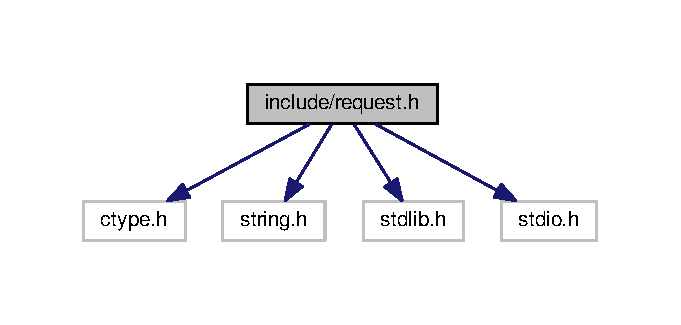
\includegraphics[width=327pt]{request_8h__incl}
\end{center}
\end{figure}
\subsection*{Classes}
\begin{DoxyCompactItemize}
\item 
struct \hyperlink{structRequest}{Request}
\begin{DoxyCompactList}\small\item\em defines a \hyperlink{structRequest}{Request} data type \end{DoxyCompactList}\end{DoxyCompactItemize}
\subsection*{Functions}
\begin{DoxyCompactItemize}
\item 
\hyperlink{structRequest}{Request} \hyperlink{request_8h_abb53a2add3eeca191b54bc374fe3e696}{parse\+Request} (const char $\ast$msg\+Str)
\begin{DoxyCompactList}\small\item\em Parsing string into \hyperlink{structRequest}{Request} structure. \end{DoxyCompactList}\item 
void \hyperlink{request_8h_a258bec69027196454ff82f1ba21f5c08}{print\+Request} (\hyperlink{structRequest}{Request} $\ast$req)
\begin{DoxyCompactList}\small\item\em Printing \hyperlink{structRequest}{Request} structure. \end{DoxyCompactList}\item 
void \hyperlink{request_8h_ab87e6408e088d61869ef3ae222064771}{parse\+Http\+Request} (const char $\ast$msg\+Str)
\begin{DoxyCompactList}\small\item\em Parsing user string request into standart Http request. \end{DoxyCompactList}\end{DoxyCompactItemize}


\subsection{Detailed Description}
\hyperlink{structRequest}{Request} type and its parsing. 



\subsection{Function Documentation}
\index{request.\+h@{request.\+h}!parse\+Http\+Request@{parse\+Http\+Request}}
\index{parse\+Http\+Request@{parse\+Http\+Request}!request.\+h@{request.\+h}}
\subsubsection[{\texorpdfstring{parse\+Http\+Request(const char $\ast$msg\+Str)}{parseHttpRequest(const char *msgStr)}}]{\setlength{\rightskip}{0pt plus 5cm}void parse\+Http\+Request (
\begin{DoxyParamCaption}
\item[{const char $\ast$}]{msg\+Str}
\end{DoxyParamCaption}
)}\hypertarget{request_8h_ab87e6408e088d61869ef3ae222064771}{}\label{request_8h_ab87e6408e088d61869ef3ae222064771}


Parsing user string request into standart Http request. 


\begin{DoxyParams}{Parameters}
{\em msg\+Str} & -\/ non http string \\
\hline
\end{DoxyParams}
\index{request.\+h@{request.\+h}!parse\+Request@{parse\+Request}}
\index{parse\+Request@{parse\+Request}!request.\+h@{request.\+h}}
\subsubsection[{\texorpdfstring{parse\+Request(const char $\ast$msg\+Str)}{parseRequest(const char *msgStr)}}]{\setlength{\rightskip}{0pt plus 5cm}{\bf Request} parse\+Request (
\begin{DoxyParamCaption}
\item[{const char $\ast$}]{msg\+Str}
\end{DoxyParamCaption}
)}\hypertarget{request_8h_abb53a2add3eeca191b54bc374fe3e696}{}\label{request_8h_abb53a2add3eeca191b54bc374fe3e696}


Parsing string into \hyperlink{structRequest}{Request} structure. 


\begin{DoxyParams}{Parameters}
{\em msg\+Str} & -\/ user request \\
\hline
\end{DoxyParams}
\begin{DoxyReturn}{Returns}
parsed request type from string 
\end{DoxyReturn}
\index{request.\+h@{request.\+h}!print\+Request@{print\+Request}}
\index{print\+Request@{print\+Request}!request.\+h@{request.\+h}}
\subsubsection[{\texorpdfstring{print\+Request(\+Request $\ast$req)}{printRequest(Request *req)}}]{\setlength{\rightskip}{0pt plus 5cm}void print\+Request (
\begin{DoxyParamCaption}
\item[{{\bf Request} $\ast$}]{req}
\end{DoxyParamCaption}
)}\hypertarget{request_8h_a258bec69027196454ff82f1ba21f5c08}{}\label{request_8h_a258bec69027196454ff82f1ba21f5c08}


Printing \hyperlink{structRequest}{Request} structure. 


\begin{DoxyParams}{Parameters}
{\em req} & -\/ request for print \\
\hline
\end{DoxyParams}

%--- End generated contents ---

% Index
\backmatter
\newpage
\phantomsection
\clearemptydoublepage
\addcontentsline{toc}{chapter}{Index}
\printindex

\end{document}
